\documentclass[10pt, uplatex, dvipdfmx]{jsarticle}
\usepackage{../mypackage}

\graphicspath{{../pictures}}

\setcounter{section}{5}

\begin{document}

\section{べき級数}

\subsection{級数}

数列 $\{a_n\}$ によって定まる以下の形の式を\textbf{級数}という.
\[
  \sum_{n=0}^{\infty} a_n = a_0+a_1+a_2+ \cdots + a_n + \cdots
\]
以下の $n$ 番目までの部分和 $S_n$ が収束するとき,級数 $\ds
\sum_{n=0}^{\infty} a_n$ は\textbf{収束する}という.
\[
  S_n=\sum_{k=0}^{n}a_n = a_0 + a_1 + \cdots + a_n
\]
また,$\ds \lim_{n \to \infty} S_n = \alpha$ であるとき,級数
$\ds \sum_{n=0}^{\infty}a_n$ の値は $\alpha$
であるといい,$\ds \sum_{n=0}^{\infty} a_n = \alpha$ と書く.当たり前の
ことを長々と定義しているように見えるかもしれないが,例えば
\[
  \sum_{n=0}^{\infty}  (-1)^n = 1 +(-1) + 1 + (-1) + 1 + \cdots
\]
という数列 $\{(-1)^n\}$ から定まる級数を
\[
  \left( 1 + \left(-1\right)\right) + \left(1 + \left(-1\right)\right) + \cdots = 0
\]
と見なしたり
\[
  1 + \left(-1+1\right) + \left(-1+1\right) + \cdots =1
\]
と見なしたりしていては収束先が定まらないので,「前から順番に足す」とい
う約束をしている.この定義に従えば,上の級数は収束しない.

\begin{example}\label{exmp:geo-seq}
  初項が $a$ で公比が $r$ の等比数列の $n$ 番目までの和は
  \[
    \sum_{k=0}^{n}ar^{k} =
    \begin{cases}
      \dfrac{a(1-r^{n+1})}{1-r} & (r \neq 1)\\ \\
      a(n+1) & (r =1)
    \end{cases}
  \]
  なので,等比級数 $\ds \sum_{n=0}^{\infty} a r^{n}$ は $|r|<1$ のとき収束し,その値は
  \[
    \sum_{n=0}^{\infty} ar^{n} = \frac{a}{1-r} \quad (r <1)
  \]
  である.$|r|\geqq 1$ のとき,この等比級数は発散する.
\end{example}

\newpage

\begin{remark}
以後,混乱のおそれがないところでは $\ds \sum_{n=0}^{\infty}$ を単に $\sum$ と略して書く.
\end{remark}

\begin{theorem}[\textbf{級数の和・定数倍}]\label{thm:linear} 2つの級数
  $\sum a_n, \; \sum b_n$ が収束する
  とき,任意の定数 $k, l \in \mathbb{R}$ に対して,級数
  $\ds \sum \left(k a_n+ lb_n\right)$ も収束し,以下が成り立つ.
  \[
    \sum \left( k a_n + l b_n\right)
    = k\left( \sum a_n\right) + l \left(\sum  b_n\right)
  \]
\end{theorem}

\begin{theorem}\label{thm:seq0}
  級数 $\ds \sum a_n$ が収束するなら,数
  列 $\{a_n\}$ は $0$ に収束する.
\end{theorem}

\begin{proof}
  級数 $\ds \sum  a_n$ が $\alpha$
  に収束するとし,$\ds S_n=\sum_{k=0}^{n}a_n$ とすると,$\ds \lim_{n \to \infty}S_n=\alpha$ だから
  \[
    a_n = S_n - S_{n-1}  \to \alpha - \alpha =0 \quad (n \to \infty)
  \]
  より,数列 $\{a_n\}$ は $0$ に収束する.
\end{proof}

定理\ref{thm:seq0}の逆は成り立たない.つまり,数列 $\{a_n\}$ が $0$ に
収束しても級数 $ \sum a_n$ が収束するとは限らない.

\begin{example}\label{exmp:harmonic}
  $a_n=\dfrac{1}{n}$ とすると,数列 $\{a_n\}$ は $0$ に収束する.一方,任意の自然数 $N$ に対して
  \[
    \sum_{n=1}^{N}a_n=\sum_{n=1}^{N} \frac{1}{n}
    \geqq \int_{1}^{N}\frac{dx}{x} = \log N \to \infty \quad (N \to \infty)
  \]
  より,級数 $\sum a_n$ は発散する.なお,部分和 $\ds \sum_{n=1}^{N} a_n$ は下図の灰色部分の面積に等しい.
  \begin{figure}[h]
    \centering
    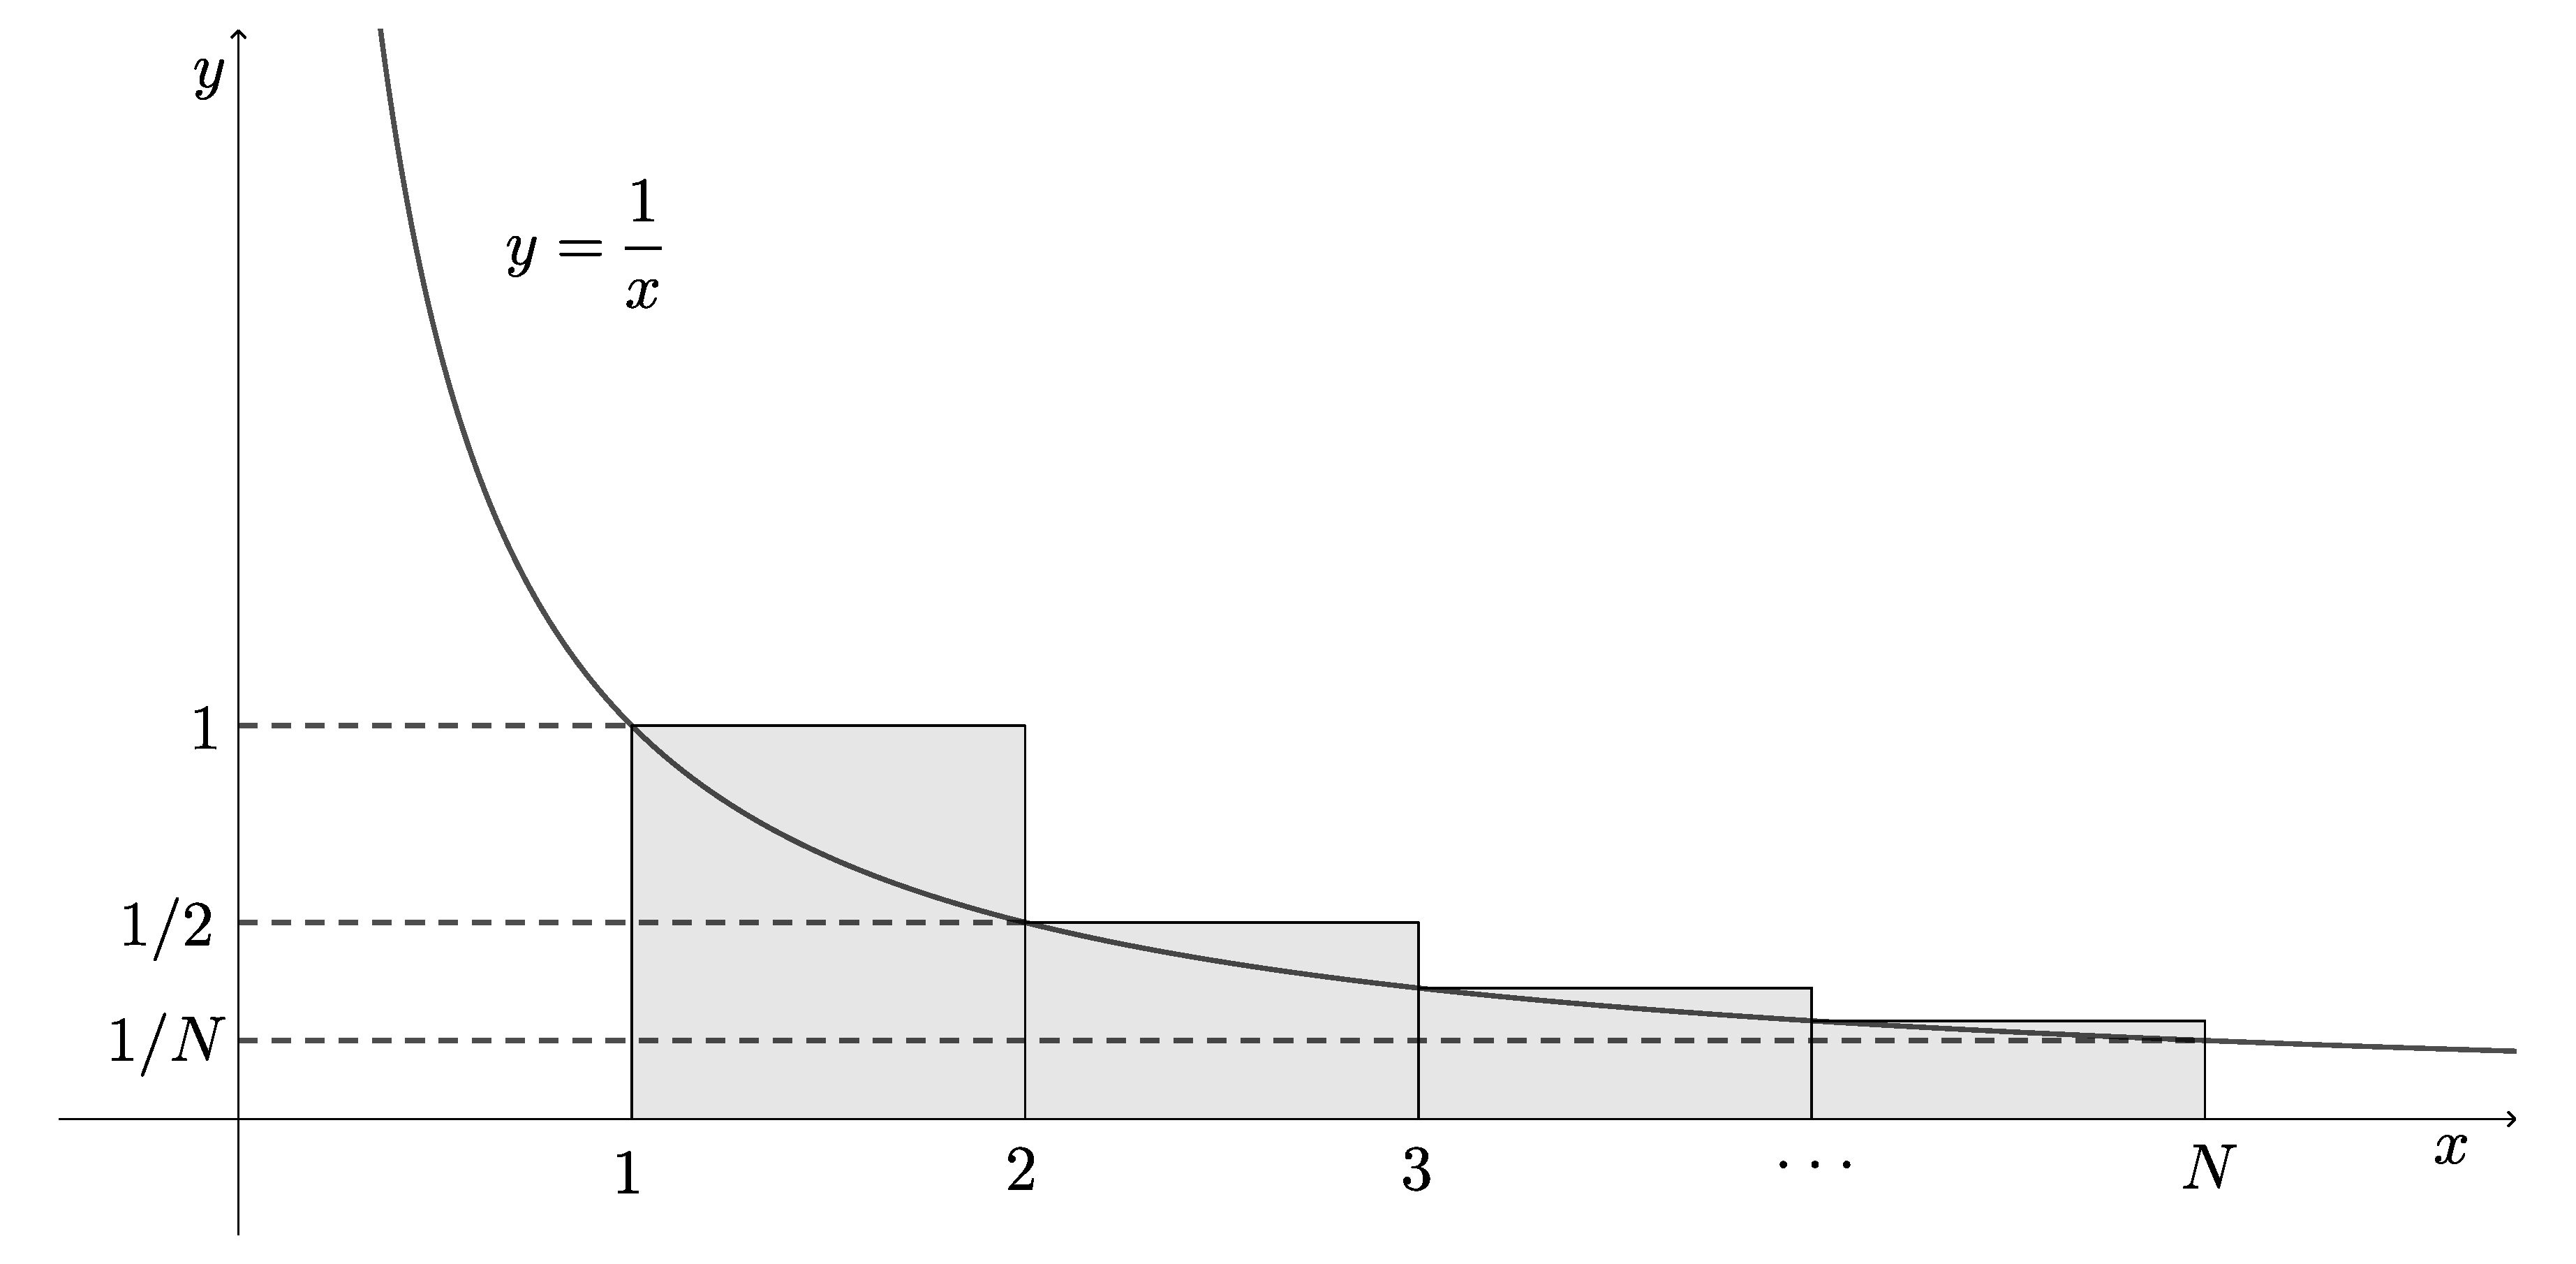
\includegraphics[width=15cm]{06/harmonic.pdf}
  \end{figure}
\end{example}

\newpage
\subsection{べき級数}

数列 $\{a_n\}$ と実数 $b$ と変数 $x$ によって
\[
  \sum_{n=0}^{\infty} a_n(x-b)^n = a_0 + a_1(x-b) + a_2(x-b)^2 + a_3(x-b)^3 + \cdots
\]
と表される級数を,$x=b$ を中心とする\textbf{べき級数}という.$t=x-b$ とおけば,この級数は
\[
  \sum_{n=0}^{\infty} a_n t^n = a_0 + a_1 t + a_2 t^2 + a_3 t^3  + \cdots
\]
と $t=0$ を中心とするべき級数に書き換えられるので,この形のべき級数が重要である.

\begin{example}
  多項式 $a_0 + a_1 x + \cdots +a_n x^n$ は,$a_{k} = 0 \; (k >n)$ とし
  て,べき級数とみなせる.
\end{example}

\begin{definition}[\textbf{Taylor 級数}]
  実数 $a$ を含む開区間 $I$ で $C^{\infty}$ 級な関数 $f$ に対し,
  \[
    \sum_{n=0}^{\infty} \frac{f^{(n)}(a)}{n!}(x-a)^n = f(a) + f'(a)(x-a) + \frac{f''(a)}{2!}(x-a)^2
    + \frac{f^{(3)}(a)}{3!}(x-a)^3 + \cdots
  \]
  を $f$ の $x=a$ を中心とする\textbf{Taylor 級数}という.
\end{definition}

関数 $f$ が $x=a$ でTaylor展開可能なとき,$a$ の近くの $x$ におい
て $f$ の $x=a$ を中心とするTaylor級数は収束し,その値は $f(x)$ に等し
い.しかしながら,一般には $f$ が $C^{\infty}$ 級であってもそのTaylor級数
と $f(x)$ が等しいとは限らない.

\begin{example}
  以下の関数 $f$ の $x=0$ を中心とするTaylor級数を考えてみよう.
  \[
    f(x) =\left\{
      \begin{array}{cc}
        e^{-\frac{1}{x^2}} & (x \neq 0)\\
        0 & (x=0)
      \end{array}
    \right.
  \]
  まず,$f'(0)$ を求めよう.以下は途中で $h=\frac{1}{t}$ と変数変換している.
  \[
    f'(0)=\lim_{h \to 0} \frac{f(0+h)-f(0)}{h} = \lim_{h \to 0} \frac{e^{-\frac{1}{h^2}}}{h}
    = \lim_{t \to \pm \infty} \frac{t}{e^{t^2}} = 0
  \]
  次に,$f''(0)$ を求めよう.やはり以下でも途中で $h=\frac{1}{t}$ と変数変換している.
  \[
    f''(0) = \lim_{h \to 0} \frac{f'(0+h)-f'(0)}{h} = \lim_{h \to 0} \frac{2h^{-3}e^{-\frac{1}{h^2}}}{h}
    =\lim_{t \to \pm \infty} \frac{2t^4}{e^{t^2}} =0
  \]
  以下,同様に計算して $f(0)=f'(0)=f''(0)= f^{(3)}(0)= \cdots = 0$ とな
  ることがわかる.従って,$f$ の $x=0$ のまわりでのTaylor級数は
  \[
    \sum_{n=0}^{\infty} \frac{f^{(n)}(0)}{n!}x^n = 0 + 0x + 0x^2 + \cdots = 0
  \]
  であるが,これは明らかに $x=0$ 以外の全ての $x$ に対して $f(x)$ と等しくない.
\end{example}

\subsection{収束半径}

\begin{theorem}\label{thm:conv-seriese}
  べき級数 $\sum a_n x^n$ が $x=b \; (\neq 0)$ で収
  束するなら,$|x| < |b|$ を満たす全ての $x$ で収束する.
\end{theorem}

\begin{proof}
  級数 $\sum a_n b^n$ が収束するので,数
  列 $\{a_nb^n\}$ は $0$ に収束する.特に,数列 $\{a_n b^n\}$ は上にも
  下にも有界なので,全ての番号 $n \geq 0$ で $|a_n b^n| <M$ となる正の
  実数 $M$が存在する.このとき,各 $x$ に対して $\ds
  r=\left|x/b\right|$ とすると,
  \[
    |a_n x^n| = \left| a_n b^n \cdot \frac{x^n}{b^n}\right| \leq M r^n
  \]
  が成り立つ.従って,$|x| < |b|$ すなわち $r<1$ ならば,級数
  $\sum Mr^n$ が収束するので
  $\sum |a_n x^n|$
  も収束する.よって,$\sum  a_n x^n$ は収束す
  る.
\end{proof}

\begin{remark}
上の証明の終盤では以下の優級数定理と呼ばれる定理を使った.
\end{remark}

\begin{theorem}[\textbf{優級数定理}] 全ての $n$ で $0 \leqq a_n \leqq
  b_n$ であり,級数 $\sum b_n$ が収束するなら,級数 $\sum a_n$ も収束す
  る.このような級数 $\sum b_n$ は級数 $\sum a_n$ の\textbf{優級数}と呼ばれる.
\end{theorem}

\begin{remark}
  級数 $\sum |a_n|$ が収束するとき,級数 $\sum a_n$ は\textbf{絶対収束
    する}という.これは級数 $\sum a_n$ が収束するよりも強い条件である.
  つまり,級数 $\sum a_n$ が絶対収束するなら,$\sum a_n$ は収束する.
\end{remark}

定理\ref{thm:conv-seriese}は級数の発散を判定する以下の定理を導くこともできる.

\begin{theorem}\label{thm:div-seriese}
べき級数 $\sum a_n x^n$ が $x=b$ で発散するな
ら,$|x| > |b|$ を満たす全ての $x$ で発散する.
\end{theorem}

\begin{proof}
$|u|> |b|$ と
なる $u$ でべき級数が収束するなら,定理\ref{thm:conv-seriese}により $x=b$ でべ
き級数が収束し,$x=b$ で発散することに矛盾する.
\end{proof}


\begin{definition}[\textbf{収束半径}]
  べき級数 $\sum a_n x^n$ が $|x| < r$ のとき収束
  し,$|x|>r$ のとき発散するとき,$r$ をこのべき級数の\textbf{収束半径}と
  いう.ただし,$x=0$ でのみ収束するときは $r=0$ とし,全ての実数 $x$
  で収束するときは $r=+\infty$ と定める.
\end{definition}


\begin{remark}
  収束半径 $r$ が $0 < r < +\infty$ のとき,定
  理\ref{thm:conv-seriese}からべき級数 $\sum  a_n
  x^n$ は $|x| <r$ で収束し,$|x|>r$ で発散する.なお,$x= \pm r$ にお
  ける収束・発散は個別に調べなければわからない.
\end{remark}


\begin{example}\label{exmp:geo}
  べき級数 $\ds \sum_{n=0}^{\infty} x^n$ は $|x|<1$ で絶対収束
  し,$|x|>1$ で発散するから,その収束半径は $1$ である.なお,この場
  合 $x=\pm1$ では発散することが容易にわかる.よって,$|x|<1$ において
  以下が成り立つ.
  \[
    \sum_{n=0}^{\infty}x^n=\frac{1}{1-x}
  \]
\end{example}

\newpage

全ての $n$ で $a_n>0$ となる級数 $\sum a_n$ を\textbf{正項級数}という.

\begin{theorem}[\textbf{Cauchy の収束判定法}]
  正項級数 $\sum a_n$ に対して,$\ds \rho := \lim_{n \to \infty}
  \sqrt[n]{a_n}$ とする.$\rho <1$ なら $\sum a_n$
  は収束し,$\ds \rho >1 \; \left( \lim_{n \to \infty} \sqrt[n]{a_n} =
    \infty \text{ も含む }\right)$ なら $\sum a_n$ は発散する.
\end{theorem}

\begin{theorem}[\textbf{d'Alembert の収束判定法}]
  正項級数 $\sum a_n$
  に対して,$\ds \rho:= \lim_{n \to \infty} \frac{a_{n+1}}{a_{n}}$ とす
  る.$\rho <1$ なら $\sum a_n$
  は収束し,$\ds \rho >1 \; \left( \lim_{n \to \infty} \frac{a_{n+1}}{a_n}
    = \infty \text{ も含む } \right)$ なら $\sum a_n$ は発散する.
\end{theorem}

\begin{remark}
  Cauchy の収束判定法も d'lAmbert の収束判定法も $\rho=1$ となるときに
  は収束・発散に関して何も教えてくれない.その場合は個別に別の方法で調べなければならない.
\end{remark}

\begin{theorem}\label{thm:criterion}
  べき級数 $ \sum a_n x^n$ の収束半径を $r$ とする.
  このとき次が成り立つ.
  \begin{enumerate}[(1)]
    \setlength{\itemsep}{1zh}
  \item 極限値 $\ds l = \lim_{n \to \infty} \sqrt[n]{|a_n|}$ が存在するとき,$\ds r=\frac{1}{l}$ である.
  \item 極限値
    $\ds l = \lim_{n \to \infty} \left| \frac{a_{n+1}}{a_n}\right|$ が
    存在するとき,$\ds r=\frac{1}{l}$ である.
  \end{enumerate}
  ただし,$l=0$ のときは $r=+\infty$ であり,$l=+\infty$ のときは $r=0$ である.
\end{theorem}

\begin{proof}
  \begin{enumerate}[(1)]
    \setlength{\itemsep}{1zh}
    
  \item 実数 $x$ に対して
    $\ds \lim_{n \to \infty} \sqrt[n]{|a_n x^n|} =
    \lim_{n=\infty}\sqrt[n]{|a_n|}|x| = l |x|$ である.従って,Cauchyの
    収束判定法から
    \begin{itemize}
      \setlength{\itemsep}{1zh}
    \item $l |x| <1$ すなわち $|x| < \dfrac{1}{l}$ ならば,べき級数は絶対収束する.
    \item $l |x| >1$ すなわち $|x| > \dfrac{1}{l}$ ならば,級数
      $\sum |a_n x^n|$ は発散する.
    \end{itemize}
    よって,収束半径は $r=\dfrac{1}{l}$ である.

  \item 実数 $x$ に対して
    $\ds \lim_{n \to \infty} \left| \frac{a_{n+1}x^{n+1}}{a_n
        x^n}\right| = \lim_{n \to \infty}
    \left|\frac{a_{n+1}}{a_n}\right| |x| = l |x|$ である.従って,d'Alembertの収束判定法から
    \begin{itemize}
      \setlength{\itemsep}{1zh}
    \item $l|x| <1$ すなわち $|x| < \dfrac{1}{l}$ ならば,べき級数は絶対収束する.
    \item $l|x| >1$ すなわち $|x| > \dfrac{1}{l}$ ならば,級数 $\sum |a_n x^n|$ は発散する.
    \end{itemize}
    よって,収束半径は $r= \dfrac{1}{l}$ である.
  \end{enumerate}
\end{proof}

\begin{example}
  べき級数 $\ds \sum_{n=0}^{\infty} \frac{x^n}{n!}$ の収束半径
  は $+\infty$ である.すなわち,全ての実数 $x$ で収束する.

  実際,$\ds a_n=\frac{1}{n!}$ とおけばこのべき級数は $\ds \sum_{n=0}^{\infty} a_n x^n$ と書けるので,
  \[
    \lim_{n \to \infty} \left| \frac{a_{n+1}}{a_n}\right| = \lim_{n \to \infty} \frac{1}{n+1} = 0
  \]
  より定理\ref{thm:criterion}から収束半径は $+\infty$ である.

\end{example}

\newpage

\subsection{項別積分・項別微分}

べき級数 $\sum a_n x^n$ の収束半径が $r>0$ なら,これは開区間 $(-r,r)$ 上の関数
\[
  f(x) = \sum  a_n x^n = a_0 + a_1 x + a_2 x^2 + \cdots
\]
を定義する.このとき,$f$ は $(-r,r)$ で連続である.

\begin{theorem}[\textbf{項別積分}]\label{thm:term-int}
  べき級数 $f(x) = \sum a_n x^n$ の収束半径を $r>0$
  とする.このとき,開区間 $(-r,r)$ 上で以下が成り立つ.すなわち,右辺の収束半径は $r$ である.
  \[
    \int_{0}^{x} f(t) \ dt = \sum_{n=0}^{\infty} \frac{a_n}{n+1}x^{n+1}
  \]
\end{theorem}

\begin{theorem}[\textbf{項別微分}]\label{thm:term-diff}
  べき級数 $f(x) = \sum a_n x^n$ と
  $g(x) = \sum  na_n x^{n-1}$ に次が成り立つ.
  \begin{enumerate}[(1)]
    
  \item $g(x)$ の収束半径は $f(x)$ の収束半径に等しい.

  \item $f(x)$ の収束半径が $r>0$ のとき,$f$ は $(-r,r)$ で微分
    可能で,$f'(x) = g(x)$ である.
  \end{enumerate}
\end{theorem}

\begin{theorem}
  正の収束半径 $r$ を持つべき級数 $f(x) = \sum  a_n
  x^n$ は $(-r,r)$ で $C^{\infty}$ 級である.
\end{theorem}
\begin{proof}
  定理\ref{thm:term-diff}より $f'(x) = \sum  n a_n
  x^{n-1}$ であり,その収束半径も $r$ である.よって,定
  理\ref{thm:term-diff}を繰り返し適用して,$f$ は何回でも微分できること
  が示せる.
\end{proof}

\begin{theorem}\label{thm:coeff}
  べき級数 $f(x) = \sum  a_n x^n$ が正の収束半
  径 $r$を持つとき,各 $n=0,1,2,\ldots$ に対して以下が成り立つ.
  \[
    a_n = \frac{f^{(n)}(0)}{n!}
  \]
\end{theorem}
\begin{proof}
  $f$ に定理\ref{thm:term-diff}を繰り返し適用して
  \[
    f^{(n)}(x) = n! a_n + \left( (n+1)n \cdots  2\right)a_{n+1} x + \left( (n+2)(n+1)\cdots 3\right) a_{n+2} x^2 + \cdots
  \]
  だから,これに $x=0$ を代入して $f^{(n)}(0) = n! a_n$ を得る.
\end{proof}

\begin{theorem}[\textbf{べき級数展開の一意性}]\label{thm:unique-seriese}
  $C^{\infty}$ 級関数 $f$ が,正の収束半径を持つべき級数として
  \[
    f(x) = \sum  a_n x^n = \sum b_n x^n
  \]
  と2通りに表せたとき,各 $n=0,1,2,\ldots$ に対して $a_n=b_n$ である.
\end{theorem}

\begin{proof}
  定理\ref{thm:coeff}より,各 $n=0,1,2,\ldots$ に対して
  $\ds a_n = \frac{f^{(n)}(0)}{n!} =b_n$ である.
\end{proof}

\newpage

\subsection{Taylor 展開}

実数 $a$ の近くで $C^{\infty}$ 級な関数 $f$ の $n$ 次剰余項
\[
  R_n(x) = f(x) -\sum_{n=0}^{n-1}\frac{f^{(k)}(a)}{k!}(x-a)^{n-1}
\]
が $n \to \infty$ のときに $0$ に収束すると
き,$f$ は $x=a$ で\textbf{Taylor展開可能}であるといい,そのTaylor級
数を $f$ の $x=a$ での\textbf{Taylor展開}という.このとき
\[
  f(x) = \sum_{n=0}^{\infty} \frac{f^{(n)}(a)}{n!}(x-a)^n
\]
である.特に,$a=0$ でのTaylor展開を $f$ の\textbf{Maclaurin展開}という.

\begin{example}\label{exmp:taylor-serieses}
  代表的なMaclaurin展開をいくつか挙げておく.
  \[
    \begin{aligned}
      e^x &= \sum \frac{x^n}{n!} = 1 + x +
            \frac{x^2}{2!} + \frac{x^3}{3!} + \cdots \quad (-\infty < x <
            \infty)\\
      \sin x & = \sum (-1)^n \frac{x^{2n+1}}{(2n+1)!}
               = x - \frac{x^3}{3!} + \frac{x^5}{5!} -\frac{x^7}{7!} + \cdots \quad (-\infty < x < \infty)\\
      \cos x &= \sum (-1)^n \frac{x^{2n}}{(2n)!}
               = 1 - \frac{x^2}{2!} + \frac{x^4}{4!}-\frac{x^6}{6!}+\cdots \quad (-\infty < x < \infty)\\
      (1+x)^{a} &= \sum \binom{a}{n}x^n = 1 + \binom{a}{1}x + \binom{a}{2}x^2
                  + \binom{a}{3}x^3 + \cdots \quad (-1 < x < 1)
        \end{aligned}
      \]
      ただし,最後の級数の係数は一般化二項係数である.
      \[
        \binom{a}{k} := \frac{\overbrace{a(a-1)\cdots(a-k+1)}^{k \text{ 個 }}}{n!}, \qquad \binom{a}{0}:=1
      \]
    \end{example}


\begin{example}\label{exmp:log-taylor}
  例\ref{exmp:geo}のべき級数 $\sum  x^n$ の収束半径
  は $1$ である.従って,$|x|<1$ において
  \[
    \frac{1}{1-x} = \sum x^n = 1 + x + x^2 + x^3 + \cdots 
  \]
  である.べき級数展開の一意性(定理\ref{thm:unique-seriese})からこれは関数 $
  f(x)=\dfrac{1}{1-x}$ のMaclaurin展開でもある.また,$|x|<1$ のと
  き,$|-x|<1$ だから
  \[
    f(-x) = \frac{1}{1+x} = \sum (-x)^n = 1 -x + x^2 - x^3 + \cdots 
  \]
  であり,最右辺の収束半径は $1$ である.よって,項別積分ができて(定理\ref{thm:term-int})
  \[
    \log(1+x) = \int_{0}^{x} \frac{dt}{1+t} = \sum \frac{(-1)^n}{n+1} x^{n+1}
    = x - \frac{x^2}{2} + \frac{x^3}{3} - \frac{x^4}{4} + \cdots 
  \]
  が $|x|<1$ で成り立つ.これは関数 $\log(1+x)$ のMaclaurin展開である.
  ちなみに,このMaclaurin展開は $x=1$ でも成り立つので,
  \[
    \log 2 = 1 - \frac{1}{2} + \frac{1}{3} - \frac{1}{4} + \cdots
  \]
  である.なお,$x=-1$ のとき級数は発散する.
\end{example}

\begin{example}\label{exmp:atan-taylor}
  $\tan^{-1}x$ のMaclaurin展開とその収束半径を項別積分を使って求める.

  例\ref{exmp:log-taylor}で見たように,$|x|<1$ で
  \[
    \frac{1}{1+x} = \sum (-x)^n = 1 - x + x^2 - x^3 + \cdots
  \]
  である.$|x| <1$ のとき,$|x^2|<1$ なので $x$ に $x^2$ を代入して
  \[
    \frac{1}{1+x^2} = \sum(-x^2)^n=\sum (-1)^n x^{2n}
    =1 -x^2 + x^4 - x^6 + \cdots 
  \]
  を得る.この収束半径は $1$ である.よって,項別積分ができて(定理\ref{thm:term-int})
  \[
    \tan^{-1}x = \int_{0}^{x}\frac{dt}{1+t^2} = \sum \frac{(-1)^n}{2n+1}x^{2n+1}
    = x - \frac{x^3}{3} + \frac{x^5}{5} - \frac{x^7}{7} + \cdots
  \]
  が開区間 $(-1,1)$ で成り立つ.べき級数展開の一意性(定理\ref{thm:unique-seriese})からこれ
  は $\tan^{-1}x$ のMaclaurin展開であり,定理\ref{thm:term-int}からその
  収束半径は $1$ である.
\end{example}

\begin{example}\label{exmp:int-exp-x2-taylor}
  以下の関数 $G(x)$ の Maclaulin 展開を項別積分を
  使って求める.
  \[
    G(x) := \int_{0}^{x} e^{-t^2} \ dt
  \]
  例\ref{exmp:taylor-serieses}で挙げた指数関数 $e^x$ の Maclaulin 展開の $x$ に $-t^2$ を代入して以下が得られる.
  \[
    e^{-t^2} = 1 - t^2 + \frac{t^4}{2!} - \frac{t^6}{3!} + \cdots + \frac{(-1)^n}{n!}t^{2n} + \cdots \quad (- \infty < t < \infty)
  \]
  右辺は項別積分ができる(定理\ref{thm:term-int})ので両辺を $0$ から $x$ まで積分して以下を得る.
  \begin{equation}\label{eq:G-seriese}
    G(x) = \int_{0}^{x}e^{-t^2} \ dt = x - \frac{x^3}{3} + \frac{x^5}{10} - \frac{x^7}{42} + \cdots + \frac{(-1)^n}{n! (2n+1)}x^{2n+1} + \cdots
    \quad (- \infty < x < \infty)
  \end{equation}
  べき級数の一意性(定理\ref{thm:unique-seriese})から,これは $G(x)$ の Maclaulin 展開である.\\
 

  
  ちなみに,この関数 $G(x)$ の $\ds \frac{2}{\sqrt{\pi}}$ 倍は\textbf{誤差関数 (error function)}
  と呼ばれ,$\erf(x)$ と書かれる.
  \[
    \erf (x) = \frac{2}{\sqrt{\pi}}\int_{0}^{x} e^{-t^2} \ dt 
  \]
  わざわざ $\ds \frac{2}{\sqrt{\pi}}$ 倍する理由はいずれ説明するつもり
  だが,これは初等関数(多項式,三角関数,逆三角関数,指数関数,対数関
  数,無理関数たちのある種の組み合わせとして表せる関数)でないことが知
  られている.そのため,各 $x$ での関数値を知るのも困難だが,上記の級数
  表示(\ref{eq:G-seriese})によって原理上は任意精度の近似値を計算するこ
  とができる.
\end{example}

\newpage
\subsection{(おまけ)Taylorの定理と積分}

\begin{theorem}\label{thm:taylor-int}
  $f$ を実数 $a$ を含む開区間 $I$ で $C^n$ 級な関数とする.このとき,任
  意の $x \in I$ に対して以下が成り立つ.
  \[
    f(x) = \sum_{k=0}^{n-1} \frac{f^{(k)}(a)}{k!}(x-a)^k +
    \int_{a}^{x}\frac{f^{(n)}(t)}{(n-1)!}(x-t)^{n-1} \ dt
  \]
\end{theorem}

\begin{proof}
  微分積分学の基本定理から,任意の $x \in I$ に対して
  \[
    f(x)-f(a) = \int_{a}^{x} f'(t) \ dt
  \]
  である.右辺の積分に部分積分を繰り返し適用して,以下を得る. 
  \[
    \begin{aligned}
      f(x) &= f(a) + \int_{a}^{x} \left( -(x-t)\right)' f'(t) \ dt\\
      &= f(a) + \Big[\left( -\left(x-t\right)\right)f'(t)\Big]_{t=a}^{t=x} + \int_{a}^{x} f''(t)(x-t)\ dt\\
      &= f(a) + f'(a)(x-a)+ \int_{a}^{x} \left( -\frac{(x-t)^2}{2}\right)' f''(t) \ dt\\
      &= \sum_{k=0}^{1}\frac{f^{(k)}(a)}{k!}(x-a)^k + \left[ -\frac{(x-t)^2}{2!}f''(t)\right]_{t=a}^{t=x}
      + \int_{a}^{x}\frac{f^{(3)}(t)}{2!}(x-t)^2\ dt\\
      &= \sum_{k=0}^{2}\frac{f^{(k)}(a)}{k!}(x-a)^k + \left[-\frac{(x-t)^3}{3!}f^{(3)}(t)\right]_{t=a}^{t=x}
      +\int_{a}^{x} \frac{f^{(4)}(t)}{3!}(x-t)^3 \ dt\\
      &= \sum_{k=0}^{3}\frac{f^{(k)}(a)}{k!}(x-a)^k + \left[-\frac{(x-t)^4}{4!}f^{(3)}(t)\right]_{t=a}^{t=x}
      + \int_{a}^{x} \frac{f^{(5)}(t)}{4!} (x-t)^4 \ dt\\
      &\qquad  \vdots\\
      &= \sum_{k=0}^{n-1}\frac{f^{(k)}(a)}{k!}(x-a)^k
      + \int_{a}^{x} \frac{f^{(n)}(t)}{(n-1)!}(x-t)^{n-1} \ dt
    \end{aligned}
  \]

\end{proof}

上の定理において
\[
  R_{n}(x) := \int_{a}^{x}\frac{f^{(n)}(t)}{(n-1)!}(x-t)^{n-1}\ dt
\]
を積分形の剰余項という.これは Taylor の定理における剰余項の別の表現方
法である.この定理\ref{thm:taylor-int}から Taylor の定理を導くこともできる.


\begin{theorem}[\textbf{Taylor の定理}]\label{thm:taylor}
  定理\ref{thm:taylor-int}と同じ仮定のもとで,任意の $x \in I$ に対して,
  以下を満たす実数 $c$ が存在する.
  \[
    f(x) = \sum_{k=0}^{n-1}\frac{f^{(k)}(a)}{k!}(x-a)^k
    +\frac{f^{(n)}(c)}{n!}(x-a)^n, \quad a<c<x \text{ または } x<c<a
  \]
\end{theorem}

\begin{proof}
  $a>x$ のときも同様に示せるので,$a<x$ とする.定理\ref{thm:taylor-int}から
  \[
    R_n(x):=\int_{a}^{x}\frac{f^{(n)}(t)}{(n-1)!}(x-t)^{n-1}\ dt =
    \frac{f^{(n)}(c)}{n!}(x-a)^n, \quad a<c<x
  \]
  を満たす実数 $c$ が存在することを示せばよい.$f$ は開区
  間 $I$ で $C^n$ 級なので,$f^{(n)}$ は閉区間 $[a,x]$ で連続である.従っ
  て,最大値・最小値の定理から,区間 $[a,x]$ における $f^{(n)}$ の最小
  値 $m$ と最大値 $M$ が存在するので
  \[
    \int_{a}^{x} \frac{m}{(n-1)!}(x-t)^{n-1}\ dt
    \leq R_n(x)
    \leq \int_{a}^{x} \frac{M}{(n-1)!}(x-t)^{n-1}\ dt
  \]
  である.ここで,
  \[
    \begin{aligned}
      \int_{a}^{x}\frac{m}{(n-1)!}(x-t)^{n-1}\ dt
      &= \frac{m}{(n-1)!}\left[ -\frac{(x-t)^{n}}{n}\right]_{t=a}^{t=x}
      =\frac{m}{n!}(x-a)^n\\ 
      \int_{a}^{x}\frac{M}{(n-1)!}(x-t)^{n-1}\ dt
      &=\frac{M}{(n-1)!}\left[ -\frac{(x-t)^{n}}{n}\right]_{t=a}^{t=x}=\frac{M}{n!}(x-a)^n
    \end{aligned}
  \]
  より
  \[
    m \leq \frac{n!}{(x-a)^n} R_n(x) \leq M
  \]
  である.よって,中間値の定理から
  \[
    \frac{n!}{(x-a)^n}R_n(x) =f^{(n)}(c)
  \]
  を満たす実数 $c \in (a,x)$ が存在する.これから以下を得る.
  \[
    R_n(x) = \frac{f^{(n)}(c)}{n!}(x-a)^n
  \]
\end{proof}

Taylor の定理における剰余項
\[
  R_n(x) = \frac{f^{(n)}(c)}{n!}(x-a)^n
\]
はLagrangeの剰余項と呼ばれる.



\end{document}
